\documentclass[UTF8]{book}
%\usepackage{geometry}
\usepackage{amsmath,amsthm,amssymb}
\usepackage{graphicx,mathtools,tikz,forest,float,color}
\usepackage{siunitx}
%\usepackage{circuitikz}
%\usepackage{pgfplots} 
%\pgfplotsset{width=10cm,compat=1.9} 
%\usepgfplotslibrary{external} 
%\tikzexternalize 
%\usetikzlibrary{positioning}
\usepackage{hyperref}
 \hypersetup{
 colorlinks,
 linkcolor=blue
 }
\usepackage{epigraph}						% quote
\usepackage{yfonts}							% fraktur font styles in text mode

\def\dbar{{\mathchar'26\mkern-12mu \mathrm{d}}}		% inexact differential
%\newcommand{\n}{\mathbb{N}}
%\newcommand{\z}{\mathbb{Z}}
%\newcommand{\q}{\mathbb{Q}}
%\newcommand{\cx}{\mathbb{C}}
%\newcommand{\real}{\mathbb{R}}
%\newcommand{\field}{\mathbb{F}}
%\newcommand{\ita}[1]{\textit{#1}}
%\newcommand{\com}[2]{#1\backslash#2}
%\newcommand{\oneton}{\{1,2,3,...,n\}}
%\newcommand\idea[1]{\begin{gather*}#1\end{gather*}}
%\newcommand\ef{\ita{f} }
%\newcommand\eff{\ita{f}}
%\newcommand\proofs[1]{\begin{proof}#1\end{proof}}
%\newcommand\inv[1]{#1^{-1}}
%\newcommand\setb[1]{\{#1\}}
%\newcommand\en{\ita{n }}
%\newcommand{\vbrack}[1]{\langle #1\rangle}

\newtheorem{theo}{Theorem}
\newenvironment{theorem}[2][Theorem]{\begin{trivlist}
\item[\hskip \labelsep {\bfseries #1}\hskip \labelsep {\bfseries }]}{\end{trivlist}}
\newenvironment{lemma}[2][Lemma]{\begin{trivlist}
\item[\hskip \labelsep {\bfseries #1}\hskip \labelsep {\bfseries #2.}]}{\end{trivlist}}
\newenvironment{exercise}[2][Exercise]{\begin{trivlist}
\item[\hskip \labelsep {\bfseries #1}\hskip \labelsep {\bfseries #2.}]}{\end{trivlist}}
\newenvironment{reflection}[2][Reflection]{\begin{trivlist}
\item[\hskip \labelsep {\bfseries #1}\hskip \labelsep {\bfseries #2.}]}{\end{trivlist}}
\newenvironment{proposition}[2][Proposition]{\begin{trivlist}
\item[\hskip \labelsep {\bfseries #1}\hskip \labelsep {\bfseries #2.}]}{\end{trivlist}}
\newenvironment{corollary}[2][Corollary]{\begin{trivlist}
\item[\hskip \labelsep {\bfseries #1}\hskip \labelsep {\bfseries #2.}]}{\end{trivlist}}

 
%% TOC 
%\usepackage{xcolor}
%\usepackage{mdframed}
%\usepackage{titletoc}
%\usepackage{etoolbox}
%
%
%\definecolor{secnum}{RGB}{13,151,225}
%\definecolor{ptcbackground}{RGB}{212,237,252}
%\definecolor{ptctitle}{RGB}{0,177,235}
%
%\pretocmd{\tableofcontents}{\begin{mdframed}[backgroundcolor=ptcbackground,hidealllines=true]}{}{}
%\apptocmd{\tableofcontents}{\end{mdframed}}{}{}
%\patchcmd{\tableofcontents}{\contentsname}{\color{ptctitle}\contentsname}{}{}
%
%\titlecontents{section}
%  [4em]{\sffamily}
%  {\color{secnum}\contentslabel{2.3em}\normalcolor}{}
%  {\titlerule*[1000pc]{.}\contentspage\\\hspace*{-3em}\vspace*{2pt}%
%    \color{white}\rule{\dimexpr\textwidth-20pt\relax}{1pt}}
%
%\titlecontents{lsection}
%  [5.8em]{\sffamily}
%  {\color{secnum}\contentslabel{2.3em}\normalcolor}{}
%  {\titlerule*[1000pc]{.}\contentspage\\\hspace*{-5.8em}\vspace*{2pt}%
%    \color{white}\rule{\dimexpr\textwidth-15.5pt\relax}{1pt}}
%
%\makeatletter
%\renewcommand*\l@chapter[2]{%
%  \ifnum \c@tocdepth >\m@ne
%    \addpenalty{-\@highpenalty}%
%    \vskip 1.0em \@plus\p@
%    \setlength\@tempdima{1.5em}%
%    \begingroup
%      \parindent \z@ \rightskip \@pnumwidth
%      \parfillskip -\@pnumwidth
%      \leavevmode
%      \advance\leftskip\@tempdima
%      \hskip -\leftskip
%      \colorbox{ptctitle}{\strut%
%        \makebox[\dimexpr\textwidth-2\fboxsep-7pt\relax][l]{%
%          \color{white}\bfseries\sffamily#1%
%          \nobreak\hfill\nobreak\hb@xt@\@pnumwidth{\hss #2}}}\par\smallskip
%      \penalty\@highpenalty
%    \endgroup
%  \fi}
%\makeatother
%\newcommand\PartialToC{%
%\startcontents[chapters]%
%\begin{mdframed}[backgroundcolor=ptcbackground,hidealllines=true]
%\printcontents[chapters]{l}{1}{\colorbox{ptctitle}{%
%  \parbox[t]{\dimexpr\textwidth-2\fboxsep\relax}{%
%    \strut\color{white}\bfseries\sffamily\makebox[5em]{%
%      Chapter~\thechapter\hfill}Contents}}\vskip5pt}
%\end{mdframed}%
%}

 
\usepackage{pdfpages}


\begin{document}

\date{\today}
%\titlehead{\centering\includegraphics[width=6cm]{tiger}}
\title{ Bachelor Physics Lecture Notes\\ AP3290 Thermodynamics
%SemA 2016/17
}
\author{Peilin \textsc{WU}
%-\\ -Personal Usage- \\
 \\City University of Hong Kong
 %\\ \\ AP3290 \\ Thermodynamics \\ 
 }
 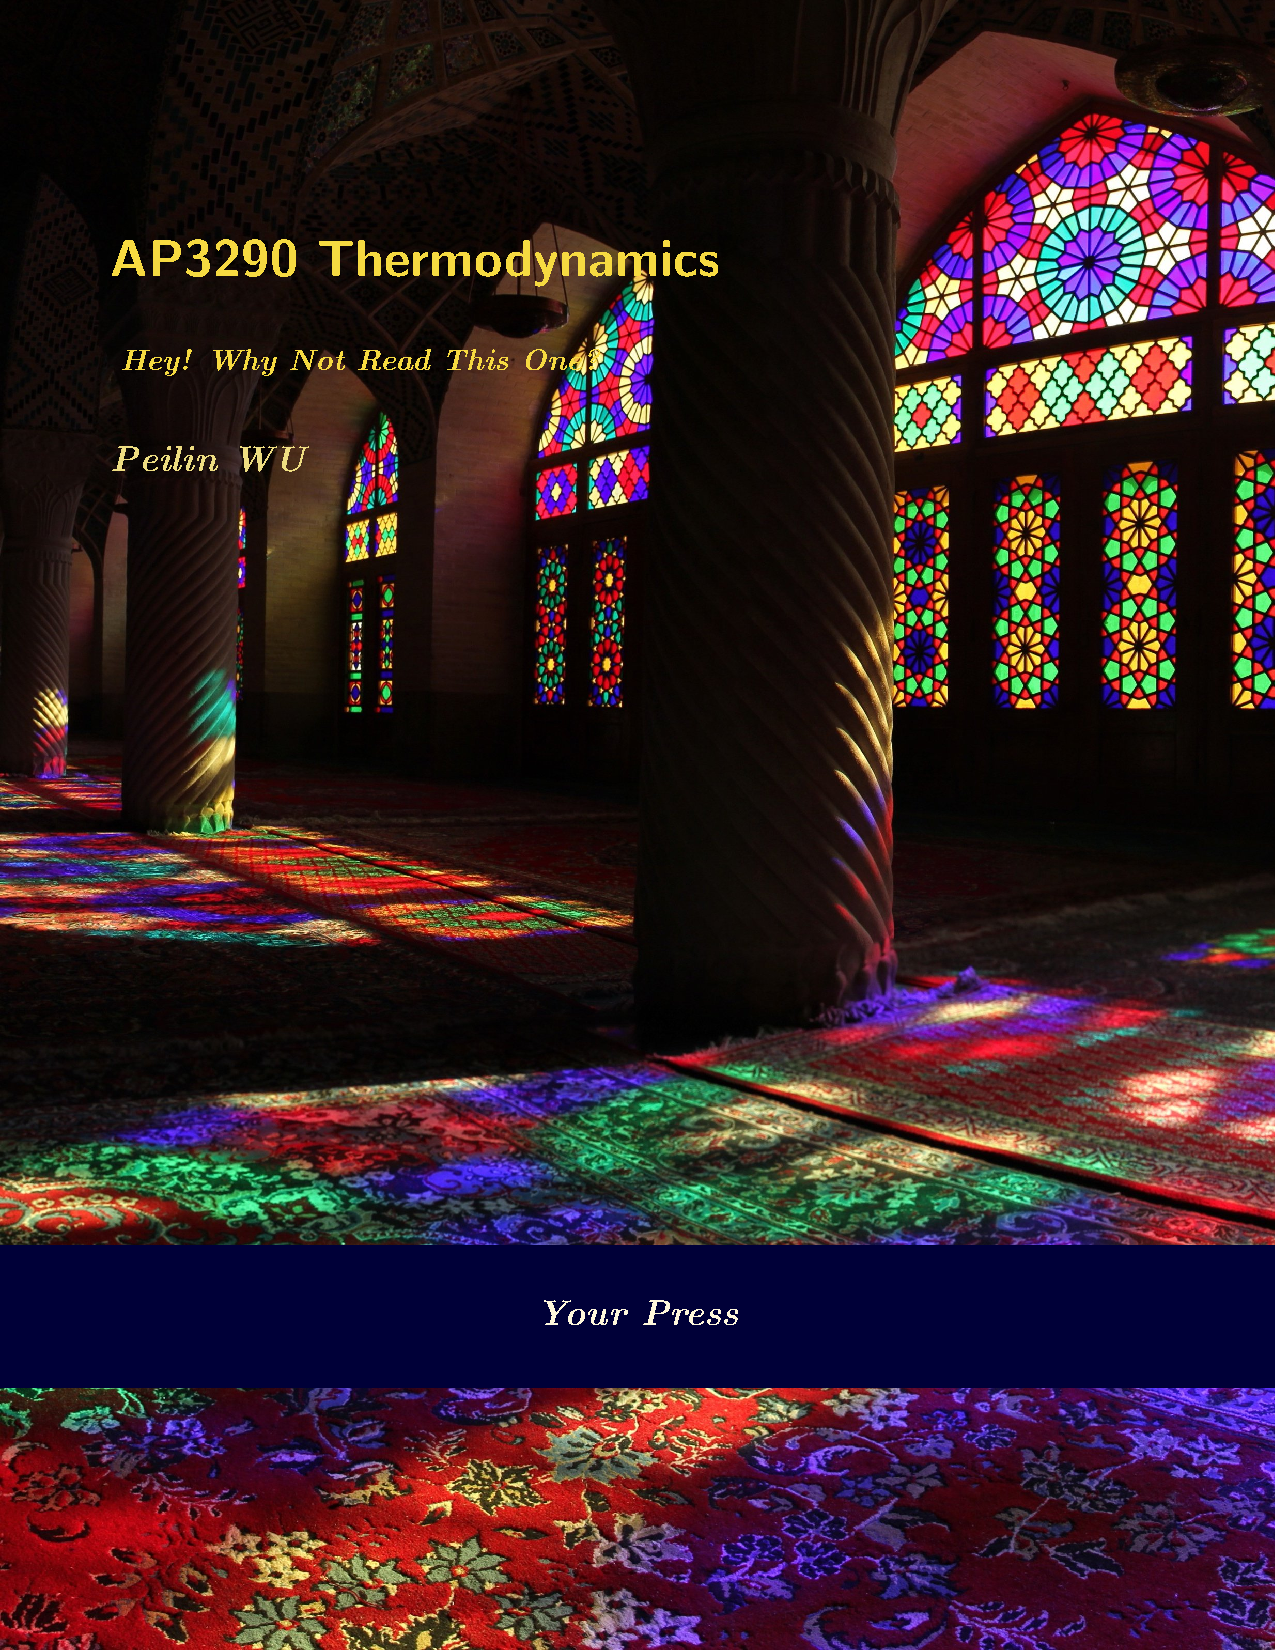
\includepdf[pages=-1]{FrontCover.pdf}
%\includegraphics{FrontCoverEbook.pdf}
\frontmatter
%\maketitle

\begin{titlepage}
    \centering
    \vfill
    {\bfseries\Large
	Bachelor Physics Lecture Notes\\ 
	AP3290 Thermodynamics
        \vskip2cm
        Peilin \textsc{WU}\\
    }    
    \vfill
    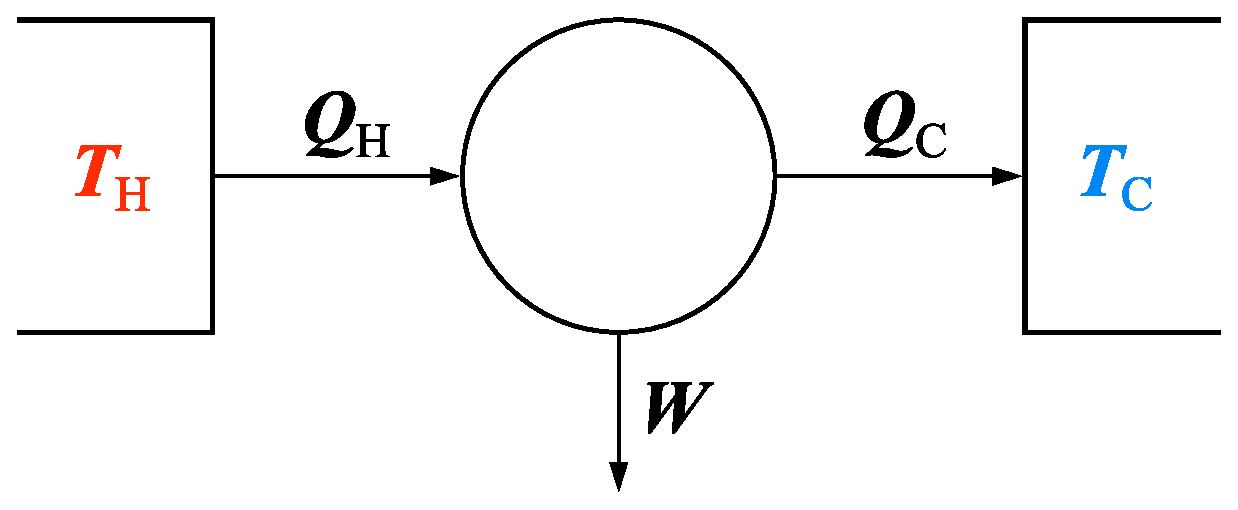
\includegraphics[width=0.5\textwidth]{Carnot_heat_engine.eps} % also works with logo.pdf
    \vfill
    \vfill
\end{titlepage}

\tableofcontents
%\pagebreak
\mainmatter
\chapter{Thermodynamic Structure}
\epigraph{\textfrak{You are very familiar with western ways, but you are too young. You go everywhere to follow the big news, but the questions you ask are too simple — sometimes na\"{i}ve. Understand, or not?}}{\textfrak{Elderly}}
\section{Laws of Thermodynamics}

 {Before we get to the first law of thermodynamics, there are some important preliminary concepts and definitions:}

\begin{theorem}[Temperature]
~  {Within a system, the temperature is a quantity which is the same for both systems when they are in equilibrium.}
\end{theorem}

\begin{theorem}[A Statistical definition of temperature]
~ Section 4.4 in \cite{blundell2009concepts}. Consider two systems are in thermal contact with each other but thermally isolated from their surroundings. Assuming the first system has the energy $E_1$ and energy $E_2$ of another system. The total energy $E=E_1+E_2$ is therefore assumed fixed. Following the below assumptions (\textsc{Ergodic hypothesis}):
%\footnote{ from Concepts in Thermal Physics}
\begin{itemize}
\item  {each one of the possible microstates of a system is equally likely to occur.}
\item  {the system's internal dynamics are such that the microstates of the system are continuously changing.}
\item  {given enough time, the system will explore all possible microstates and spend equal time in each of them.}
\end{itemize}

 {And by this, we define the microstates in each system are $\Omega _1(E_1)$ and $\Omega _2(E_2)$:}
$$\dfrac{d}{dE_1}(\Omega _1(E_1)\Omega _2(E_2))=\Omega _2(E_2)\dfrac{d\Omega _1(E_1)}{dE_1}+\Omega _1(E_1)\dfrac{d\Omega _2(E_2)}{dE_1}\dfrac{dE_2}{dE_1}=0.$$
Since the total energy $E=E_1+E_2$ is conserved, we have $dE_1=-dE_2 \implies \dfrac{dE_2}{dE_1}=-1$, therefore:
$$\dfrac{1}{\Omega _1}\dfrac{\Omega _1}{E_1}-\dfrac{1}{\Omega _2}\dfrac{\Omega _2}{E_2}=0$$
 {Hence:}
$$\dfrac{d\ln \Omega _1}{E_1}=\dfrac{d\ln \Omega _2}{E_2}$$
 Thus we choose to define temperature:
$$\boxed{\dfrac{1}{k_BT}=\dfrac{d\ln \Omega }{dE}}$$
\end{theorem}

\begin{theorem}
[Thermal Equilibrium]~  {When two systems are in thermal contact and reach a stage where no thermal changes occur, then they reach the thermal equilibrium.}
\end{theorem}

\begin{theorem}
[The Zeroth Law of Thermodynamics]~ If bodies $A$ and $B$ are each in thermal equilibrium with a third body $T$, then they are in thermal equilibrium with each other.
\end{theorem}

\subsection{The First Law of Thermodynamics}
\epigraph{The first law of thermodynamics\\
Heat is work and work is heat \\
Very good}{Flanders \& Swann}
\begin{theorem}
[The First Law of Thermodynamics]~  {Energy is conserved and heat and work are both form of energy, with mathematical description:}
$$\boxed{\Delta U=\Delta Q+\Delta W}$$
where: $U$ is the internal energy, $Q$ is the heat that flows into system and $W$ is the work done on the system.
{And by convention, we define the sign as following:}
\begin{align*}
 \textrm{for }W\ &
   \begin{dcases}
     +ve \quad  \textrm{if the work is done by environment on system}\\
     -ve \quad  \textrm{if the work is done by system on environment}
   \end{dcases}\\
 \textrm{for }Q\ &
   \begin{dcases}
     +ve \quad  \textrm{heat flow to system from environment}\\
     -ve \quad  \textrm{heat flow to environment from system}
   \end{dcases}
\end{align*}
 {or in differential form:}
$$\boxed{\mathrm{d} U=\dbar Q+\dbar W}.$$

We can see the difference of state function and process variables. $\mathrm{d}U$ indicates that $U$ is a state function which correspond to conserved potential energy, $\dbar Q$ and $\dbar W$ indicate that $Q$ and $W$ are process variables which depend explicitly upon the path.
\end{theorem}

\begin{theorem}
[Heat]~  {Heat is thermal energy in transit.}
\end{theorem}
\begin{theorem}
[Heat Capacity]~  {Heat capacity or thermal capacity is a measurable physical quantity equal to the ratio of the heat added to (or removed from) an object to the resulting temperature change.}
\[\boxed{C=\frac{dQ}{dT} \; [\si{\joule\per\kelvin}]}\]
 {For more specific situations, we also define the heat capacity per unit mass $c\,(\si{\joule\per\kelvin\per\kilo\gram})$, and molar heat capacity $C\,(\si{\joule\per\kelvin\per\mole})$}.

{Besides this, by applying a constraint to the system, we define two new quantities in case of \textbf{isochoric} (constant volume) and \textbf{isobaric} (constant pressure) process.}
$$C_V=\left(\dfrac{\partial Q}{\partial T}\right)_V,$$
$$C_p=\left(\dfrac{\partial Q}{\partial T}\right)_p,$$
{where }$C_p > C_V$ { and can be shown that later on:}
\begin{equation}\label{heat capacity}
C_p-C_V=\left[p+\left(\dfrac{\partial U}{\partial V}\right)_T\right]\left(\dfrac{\partial V}{\partial T}\right)_p=\dfrac{TV\beta _p^2}{\alpha _T }.
\end{equation}
\end{theorem}
\rule{\textwidth}{1pt}

Before, the concepts of reversibility.
And example of irreversible
\begin{enumerate}
\item Heat transfer through a finite temperature difference
\item Friction
\item Plastic deformation
\item Flow of electric current through a resistance
\item Magnetization or polarization with a hysteresis
\item Unrestrained expansion of fluids
\item Spontaneous chemical reactions
\item Spontaneous mixing of matter of varying composition/states
\end{enumerate}
{Applying the first law of thermodynamics to some special cases of ideal gases:}
\begin{itemize}
\item  {\textbf{Isobaric} (Constant $p$) Process}
$$\delta Q=nC_p\Delta T, \quad \delta W=-p\Delta V $$
\item  {\textbf{Isochoric} (Constant $V$) Process}
$$\delta W=-p \mathrm{d}V=0, \quad \delta Q=dU=nC_v\Delta T$$
\item  {\textbf{Isothermal} (Constant $T$) Process}
$$dU=0,\quad \delta Q=-\delta W=(n)RT\ln \dfrac{V_f}{V_i}$$
\begin{proof}
 {As isothermal process, $\Delta T=0$, and for ideal gas that $dU=C_VdT$, we obtain $\Delta U=0$, thus implies $\delta W=-\delta Q$.}
$$\Delta Q = \int dQ =-\int dW=\int_{V_i}^{V_f}p d V=\int_{V_i}^{V_f}\dfrac{RT}{V}dV=RT\ln \dfrac{V_f}{V_i}$$
\end{proof}
\item  {\textbf{Adiabatic} Process}
$$\delta Q=0, \,  \mathrm{d} U= \delta W  \qquad PV^{\gamma}=\mathrm{constant}$$
\begin{proof}
 {As adiabatic process which is both adiathermal and reversible, $\delta Q=0$, implies that $dU=\delta W$. And for ideal gas, $dU=C_VdT$:}
\begin{align*}
\int_{T_i}^{T_f}C_VdT&=\int_{V_i}^{V_f}-pdV=\int_{V_i}^{V_f}-\dfrac{RT}{V}dV\\
\ln \dfrac{T_f}{T_i}&=-\dfrac{R}{C_V}\ln \dfrac{V_f}{V_i}
\end{align*}
 {Assign $\gamma=C_p/C_V$, we have three constant thermal quantities:}
\begin{align*}
TV^{\gamma -1}&= {constant}\\
p^{1-\gamma}T^{\gamma}&= {constant}\\
pV^{\gamma}&= {constant}
\end{align*}
\end{proof}
\end{itemize}

\subsection{The Second Law of Thermodynamics}
\epigraph{Every mathematician knows it is impossible to understand an elementary course in thermodynamics.}{Vladimir Igorevich Arnold}
Chapter 14 -- Entropy in \cite{blundell2009concepts}.
\begin{theorem}[Clausius Inequality]
{For all thermodynamic cycles, reversible or irreversible, the Clausius inequality is valid:}
$$\oint \dfrac{\delta Q}{T}\leq 0$$
 {but for a reversible cycle, the processes can go in ``forward" or ``reverse" directions. $\delta Q$'s have opposite sign for the two directions. Therefore,}
$$\oint \left(\dfrac{\delta Q}{T}\right)_{rev}=0$$
 {therefore, for a process, the entropy change is given by: }
$$\Delta S=\int_{1}^{2}\left(\dfrac{\delta Q}{T}\right)_{rev}$$
$$\int_{1}^{2}\dfrac{\delta Q}{T}+\int_{1}^{2}\left(\dfrac{\delta Q}{T}\right)_{rev}\leq 0$$
$$dS=S_2-S_1\geq \int_{1}^{2}\left(\dfrac{\delta Q}{T}\right)$$
$$S_2-S_1=\int_{1}^{2}\left(\dfrac{\delta Q}{T}\right)+S_{gen}$$
\end{theorem}
\begin{theorem}
[Entropy]~  {Therefore, we can define this property as entropy:}
$$dS=\left(\dfrac{\delta Q}{T}\right)_{rev}\geq \dfrac{\delta Q}{T}\geq 0$$
\end{theorem}

\begin{theorem}
[Extended First Law]~  {The extended first law of thermodynamics, with the mathematical expression:}
$$\boxed{dU=TdS-pdV}$$
$$dU=\left(\dfrac{\partial U}{\partial S}\right)_VdS+\left(\dfrac{\partial U}{\partial V}\right)_SdV$$
 {with the previous statement of the second law of thermodynamics, there are three different aspects:}
\begin{itemize}
\item  {\textbf{Clausius' statement of the second law of thermodynamics}: No process is possible whose sole result is the transfer of heat from a colder to a hotter body.}
\item  {\textbf{Kelvin's statement of the second law of thermodynamics}: No process is possible whose sole result is the complete conversion of heat into work.}
\end{itemize}
\end{theorem}
\rule{\textwidth}{1pt}
{However, it is possible to construct the entropy in the terms of the statistic views.}
\begin{theorem}
[Statistical Definition of Entropy]~  { Using $dS=\delta Q/T$, we can define the entropy via statistics. As the first law of thermodynamics implies:}
$$T=\left(\dfrac{\partial U}{\partial S}\right)_V \qquad \dfrac{1}{T}\left(\dfrac{\partial S}{\partial U}\right)_V$$
 {As we recall the statistical definition of temperature:}
$$\dfrac{1}{k_BT}=\dfrac{d\ln \Omega}{dE}$$
 {we can determine the statistical definition of entropy:}
$$\boxed{S=k_B\ln \Omega }$$
 {And for more generality, here are Gibb's expression of the entropy:}
$$S=-k_B\sum_{i}P_i\ln P_i$$
 {where $P_i=\dfrac{n_i}{N}$}
\end{theorem}

\subsection{The Third Law of Thermodynamics}
\epigraph{Zeroth: You must play the game.\\
First: You can't win.\\
Second: You can't break even.\\
Third: You can't quit the game.}{}
\begin{theorem}
[Nernst's statement of the third law]~  {Near absolute zero, all reactions in a system in the internal equilibrium take place with no change in entropy.}
\end{theorem}

\begin{theorem}
[Planck's statement of the third law]~  {The entropy of all systems in internal equilibrium is the same at absolute zero, and may be taken to be zero.}
\end{theorem}

\begin{theorem}
[Simon's statement of the third law]~  {The contribution to the entropy of a system by each aspect of the system which is in internal thermodynamic equilibrium tended to zero as $T \rightarrow 0$.}
\end{theorem}

\section{Thermodynamic Systems}
\begin{itemize}
\item{ {\textbf{Unary vs. Multicomponent}}}
 { with one or more component.}
\item{ {\textbf{Homogeneous vs. Heterogeneous}}}
 { with single phase or multiple phases}
\item{ {\textbf{Closed vs. Open}}}
 { with particle exchange with the environment or not}
\item{ {\textbf{Nonreacting vs. Reacting}}}
 { with chemical reaction or not}
\item{ {\textbf{Otherwise simple vs. Complex}}}
 { with external field (any gravitational, electrical, magnetic, or surface influence)}
\end{itemize}

\section{Thermodynamic Properties}
\subsection{Thermal Variables}
\begin{itemize}
\item \textbf{Internal energy $U$}
$$dU=TdS-pdV$$
$$T=\left(\dfrac{\partial U}{\partial S}\right)_V \qquad p=-\left(\dfrac{\partial U}{\partial V}\right)_S$$
\item \textbf{Enthalpy $H$} \cite{schroeder1999introduction}
$$dH=TdS+Vdp$$
$$T=\left(\dfrac{\partial H}{\partial S}\right)_p \qquad V=\left(\dfrac{\partial H}{\partial p}\right)_S$$
\item \textbf{Helmholtz function $F$}
$$dF=-SdT-pdV$$
$$S=-\left(\dfrac{\partial F}{\partial T}\right)_V \qquad p=-\left(\dfrac{\partial F}{\partial V}\right)_T$$
\item \textbf{Gibbs function $G$}
$$dG=-SdT+Vdp$$
$$S=-\left(\dfrac{\partial G}{\partial T}\right)_p \qquad V=\left(\dfrac{\partial G}{\partial p}\right)_T$$
\item \textbf{Chemical potential $\mu$}

\begin{theorem}
[Chemical Potential]~  {Notice that in a dynamic process, adding or subtracting particles in a system will change the internal energy thus we have to modify the first law and the second law of thermodynamics with an extra term:}
$$dU=TdS-pdV+\sum_i\mu _idN_i$$
 {where $N$ is the number of the particles in the system. This means that we can write an expression $\mu $ as a partial differential of $U$ as follows:}
$$\mu =\left(\dfrac{\partial U}{\partial N}\right)_{S,V}$$
 {However, keeping $S$ and $V$ constant is a difficult constraint to apply, so it is convenient to consider other thermodynamics potentials.}
\begin{align*}
dF&=-pdV-SdT+\sum_i\mu _idN_i \implies \mu _i =\left(\dfrac{\partial F}{\partial N}\right)_{V,T,i}\\
dG&=Vdp-SdT+\sum_i\mu _idN_i \implies \mu _i =\left(\dfrac{\partial G}{\partial N}\right)_{p,T,i}
\end{align*}
\end{theorem}
\end{itemize}

\section{Thermodynamic Relationships}
\begin{theorem}
[Coefficient Relations]~  {Given any thermodynamic relation among differentials of state functions, the coefficient relations can be written down by inspection. For a state function Z, if $dZ=MdX+NdY$, then:}
$$M=\left( \frac{\partial Z}{\partial Y}\right)_{X}\qquad N=\left( \frac{\partial Z}{\partial X}\right)_{Y}$$
\end{theorem}
\begin{theorem}
[Maxwell's Relation]~  {For any state function $f$ is a function of variables $x$ and $y$. Then we have:}
$$df=\left(\dfrac{\partial f}{\partial x}\right)_ydx+\left(\dfrac{\partial f}{\partial y}\right)_xdy$$
$$\left(\dfrac{\partial ^2 f}{\partial x\partial y }\right)=\left(\dfrac{\partial ^2 f}{\partial y\partial x }\right)$$
$$F_x=\left(\dfrac{\partial f}{\partial x}\right)_y \ and \ F_y=\left(\dfrac{\partial f}{\partial y}\right)_x$$
$$\left(\dfrac{\partial F_y}{\partial x}\right)=\left(\dfrac{\partial F_x}{\partial y}\right)$$
 {Therefore, for the above four thermodynamic potentials $U$, $H$, $F$, and $G$, we can apply the theorem.}
$$\left(\dfrac{\partial T}{\partial V}\right)_S=-\left(\dfrac{\partial p}{\partial S}\right)_V \qquad \left(\dfrac{\partial T}{\partial p}\right)_S=\left(\dfrac{\partial V}{\partial S}\right)_p$$
$$\left(\dfrac{\partial S}{\partial V}\right)_T=\left(\dfrac{\partial p}{\partial T}\right)_V \qquad \left(\dfrac{\partial S}{\partial p}\right)_T=-\left(\dfrac{\partial V}{\partial T}\right)_p$$
\end{theorem}
\begin{proof}
 {Here is an elegant derivation of the Maxwell's relation by using the Jocabian. Consider a cyclic process that can be described in both $T-S$ and $p-V$ planes. The internal energy $U$ is a state function and therefore is path independent, which implies that $\oint dU=0$. Therefore:}
$$\oint pdV=\oint TdS$$
$$\iint dpdV=\iint dTdS$$
 {but we can also write as following:}
$$\iint dpdV\dfrac{\partial (T,S)}{\partial (p,V)}=\iint dTdS \implies \dfrac{\partial (T,S)}{\partial (p,V)}=1$$
$$\dfrac{\partial (T,S)}{\partial (x,y)}=\dfrac{\partial (p,V)}{\partial (x,y)}$$
 {where $(x,y)$ are taken as $(T,p)$, $(T,V)$, $(p,S)$, and $(S,V)$.}
\end{proof}

 {Note, here is an memorize technique. For each Maxwell's relations, it is in of the form:}
$$\left(\dfrac{\partial \ast}{\partial \ddagger}\right)_\star=\pm \left(\dfrac{\partial \dagger}{\partial \star}\right)_\ddagger$$
 {where $\ast $ and $\star$, $\dagger$ and $\ddagger$ are conjugate variables, and you always have a minus sign when $V$ and $T$ are on the same side of equation.}

\begin{theorem}
[Common Usage of Maxwell's Relation]~  {Utilizing the Maxwell's relations, we can achieve that to obtain expression only in terms of the experimental variables:}
\begin{itemize}
\item  {Write down a thermodynamic potential $f$ in terms of particular variables $f(x,y)$:}
$$df=\left(\dfrac{\partial f}{\partial x}\right)_ydx+\left(\dfrac{\partial f}{\partial y}\right)_xdy$$
\item  {Use Maxwell's relations to transform the partial differential you start with into a more convenient one.} 
\item  {Invert a Maxwell's relation using the reciprocal theorem:}
$$\left(\dfrac{\partial x}{\partial z}\right)_y=\left(\dfrac{\partial z}{\partial x}\right)_y^{-1}$$
\item  {Combine partial differential using the reciprocity theorem:}
$$\left(\dfrac{\partial x}{\partial y}\right)_z\left(\dfrac{\partial y}{\partial z}\right)_x\left(\dfrac{\partial z}{\partial x}\right)_y=-1$$
\item  {Identify a heat capacity:}
$$\dfrac{C_V}{T}=\left(\dfrac{\partial S}{\partial T}\right)_V \quad \dfrac{C_p}{T}=\left(\dfrac{\partial S}{\partial T}\right)_p$$
\item  {Identify a generalized susceptibility:}\\
 {the isoabric expansivity $\beta _p$:}
$$\beta _p =\dfrac{1}{V}\left(\dfrac{\partial V}{\partial T}\right)_p$$
 {the adiabatic expansivity $\beta_S$:}
$$\beta _S =\dfrac{1}{V}\left(\dfrac{\partial V}{\partial T}\right)_S$$
 {the isothermal compressibility $\alpha _T$:}
$$\alpha _T =-\dfrac{1}{V}\left(\dfrac{\partial V}{\partial p}\right)_T$$
 {the adiabatic compressibility $\alpha _S$:}
$$\alpha _S =-\dfrac{1}{V}\left(\dfrac{\partial V}{\partial p}\right)_S$$
\end{itemize}
\end{theorem}

\section{Equilibrium}
\begin{theorem}
[General Criterion for Equilibrium]~  {An equilibrium state is:}
\begin{itemize}
\item  {A state of rest: time independence}
\item  {A state of balance: will restore to the equilibrium if perturbed from the equilibrium state}
\end{itemize}
\end{theorem}

\begin{theorem}
[Isolated Theorem]~  {If a system is in equilibrium both internally and with its surroundings, then isolating it from its surroundings produce no change in the internal state of the system. - J. Willard Gibbs}
\end{theorem}

\begin{theorem}
[The Extremum Principle]~  {In an isolated system the equilibrium state is the state that has the maximum value of entropy that the system can exhibit.}
\end{theorem}

 {The following is a example of the equilibrium in a unary two phase $(\alpha , \beta)$, nonreacting otherwise simple system. Within it, each phase has its own set of extensive and intensive properties. All extensive properties of the system id the sum of the values of the individual phases. The boundary is a natural boundary and each phase is an open system.}
 
 {First, we express the total entropy of the system as:}
$$dS'_{sys}=dS'^\alpha +dS'^\beta $$
 {From the combined $1^{st}$ and $2^{nd}$ law:}
$$dU'^\alpha =T^\alpha dS'^\alpha -P^\alpha dV'^\alpha +\mu ^\alpha dn^\alpha $$
 {divided by $T^\alpha $}
$$dS'^\alpha =\dfrac{1}{T^\alpha }dU'^\alpha +\dfrac{p^\alpha }{T^\alpha }dV'^\alpha -\dfrac{\mu ^\alpha }{T^\alpha }dn^\alpha $$
$$dS'^\beta  =\dfrac{1}{T^\beta }dU'^\beta +\dfrac{p^\beta }{T^\beta }dV'^\beta -\dfrac{\mu ^\beta }{T^\beta }dn^\beta $$
 {Since the total internal energy for an isolated system is conserved and constant volume with a rigid boundary and no mass flow for impermeable boundary.}
$$dU'^\alpha=-dU'^\beta \quad dV'^\alpha=-dV'^\beta \quad dn'^\alpha=-dn'^\beta $$
$$dS'_{sys}=\left(\dfrac{1}{T^\alpha }-\dfrac{1}{T^\beta }\right)dU'^\alpha+\left(\dfrac{p^\alpha }{T^\alpha }-\dfrac{p^\beta }{T^\beta }\right)dV'^\alpha-\left(\dfrac{\mu ^\alpha }{T^\alpha }-\dfrac{\mu ^\beta }{T^\beta }\right)dV'^\alpha $$
 {the system total entropy reach the maximum only when the coefficients reach zero. Therefore, simultaneously: $T^\alpha =T^\beta $, $p^\alpha =p^\beta $, $\mu ^\alpha =\mu ^\beta $}
 {For an alternative criterion for equilibrium based on the other energy functions: }
\begin{itemize}
\item  {For the properties constrained to constant $S,P$, equilibrium yield the minimized properties $H$}
\item  {For the properties constrained to constant $T,V$, equilibrium yield the minimized properties $F$}
\item  {For the properties constrained to constant $T,P$, equilibrium yield the minimized properties $G$}
\end{itemize}

\chapter{Cases Studies and Applications}
\epigraph{\textfrak{Were it to benefit my country I would lay down my life;\\
What then is risk to me?}}{\textfrak{Elderly}}
\section{Unary Heterogeneous System}
\subsection{The Gibbs-Duhem Equation}
$$d\mu =-sdT+vdp$$
 {From this equation we can see the relationship of those variables:}
$$\left(\dfrac{\partial \mu }{\partial p}\right)_T=v \qquad \left(\dfrac{\partial \mu}{\partial T}\right)_p=-s$$
\subsection{Chemical Potential Surfaces}

\subsection{Gibbs Phase Rule}
\subsection{Clausius-Clapeyron Equation}
\section{Statistical Thermodynamics}
\section{Maxwell-Boltzmann Distribution}
\subsection{Kinetic Theory for Gases}
\begin{itemize}
\item Internal Energy for Ideal Gases

 {In here, we give the derivation of the internal energy for ideal gases: }
$$U=\dfrac{3}{2}nRT$$
\begin{proof}
 {Consider a cubic box with length $L$ is full with monoatomic gas particles bounding off the wall and bumping into each other. First, let's look at the $x$-direction momentum:}
$$\Delta p_x=(-mv_x)-(mv_x)=-2mv_x$$
 {and the momentum change of the wall is $2mv_x$, and the time interval for each collision assumed to be $\Delta t=\dfrac{2L}{v_x}$, therefore, the rate of change of momentum is:}
$$\dfrac{\Delta p_x}{\Delta t}=\dfrac{mv_x^2}{L}$$
 {therefore, take the pressure on the wall arising from all particle into consideration:}
$$p=\dfrac{F_x}{L^2}=\dfrac{\sum_{i=1}^{N}\dfrac{mv_{xi}^2}{L}}{L}=\dfrac{m}{L^3}\sum_{i=1}^{N}v_{xi}^2=\dfrac{m}{L^3}nN_A\bar{v_x^2}=\dfrac{nN_Am\bar{v_x^2}}{V}$$
 {By writing $N=nN_A$, and let $\bar{v_x^2}$ represent the average of $v_{xi}^2$, and we notice that:}
$$\bar{v_x^2}=\dfrac{\bar{v^2}}{3}$$
$$pV=\dfrac{1}{3}nN_Am\bar{v^2}$$
 {If the gas molecules are far away and not interacting, U only arise from the transnational kinetic energy of gas molecules.}
$$U=\sum K.E.=nN_A\dfrac{1}{2}mv_{rms}^2=\dfrac{3}{2}pV=\dfrac{3}{2}nRT$$
\end{proof}
\item  {The Velocity Distribution}

\item  {The Speed Distribution}
\item 
\end{itemize}

\section{Quantum Statistical Thermodynamics}
\subsection{Bose-Einstein distributions}
\subsection{Fermi-Dirac distributions}
%\pagebreak
\newpage

\chapter{Supplementary Materials}
\section{Heat capacity}
In Equation \ref{heat capacity}, we have
$$C_p-C_V=\left[p+\left(\dfrac{\partial U}{\partial V}\right)_T\right]\left(\dfrac{\partial V}{\partial T}\right)_p=\dfrac{TV\beta _p^2}{\alpha _T }$$
\begin{proof}
\textsf{Section 11.3 \cite{blundell2009concepts}} {In general, the internal energy will be a function of temperature and volume, so that we can write $U=U(T,V)$. Hence a small change in $U$ can be related to changes in $T$ and $V$ by:}
$$dU=\left(\dfrac{\partial U}{\partial T}\right)_VdT+\left(\dfrac{\partial U}{\partial V}\right)_TdV$$
 {the first law of thermodynamics yields:}
$$dQ=dU+pdV$$
$$dQ=\left(\dfrac{\partial U}{\partial T}\right)_VdT+\left[\left(\dfrac{\partial U}{\partial V}\right)_T+p\right]dV$$
$$\dfrac{dQ}{dT}=\left(\dfrac{\partial U}{\partial T}\right)_V+\left[\left(\dfrac{\partial U}{\partial V}\right)_T+p\right]\dfrac{dV}{dT}$$
 {recall the definition of the heat capacity and note the constraint.}
\begin{align*}
C_V&=\left(\dfrac{\partial Q}{\partial T}\right)_V=\left(\dfrac{\partial U}{\partial T}\right)_V\\
C_p&=\left(\dfrac{\partial Q}{\partial T}\right)_p=\left(\dfrac{\partial U}{\partial T}\right)_V+\left[\left(\dfrac{\partial U}{\partial V}\right)_T+p\right]\left(\dfrac{\partial V}{\partial T}\right)_p\\
C_p-C_V&=\left[p+\left(\dfrac{\partial U}{\partial V}\right)_T\right]\left(\dfrac{\partial V}{\partial T}\right)_p
\end{align*}
 {therefore, we prove the first part of this relation. 
 
 \textsf{Example 16.5 \cite{blundell2009concepts}}
 And for the second part, we need to use the Maxwell's relation. Considering $S=S(T,V)$ allow us to write down immediately that:}
$$dS=\left(\dfrac{\partial S}{\partial T}\right)_VdT+\left(\dfrac{\partial S}{\partial V}\right)_TdV$$
 {Differentiating this equation w.r.t $T$ at constant $p$ yields:}
$$\left(\dfrac{\partial S}{\partial T}\right)_p=\left(\dfrac{\partial S}{\partial T}\right)_V+\left(\dfrac{\partial S}{\partial V}\right)_T\left(\dfrac{\partial V}{\partial T}\right)_p$$
 {Now the first two terms can be replaced by $C_p/T$ and $C_V/T$ respectively, while use of a Maxwell's relation and a partial differential identity:}
$$\left(\dfrac{\partial x}{\partial y}\right)_z=-\left(\dfrac{\partial x}{\partial z}\right)_y\left(\dfrac{\partial z}{\partial y}\right)_x$$
 {This yields:}
\[\left(\dfrac{\partial S}{\partial V}\right)_T=\left(\dfrac{\partial p}{\partial T}\right)_V=-\left(\dfrac{\partial p}{\partial V}\right)_T\left(\dfrac{\partial V}{\partial T}\right)_p\]
and combine the definition of the heat capacity:$C_p-C_V=\dfrac{TV\beta _p^2}{\alpha _T }.$
\end{proof}

\bibliographystyle{alpha}
\bibliography{3290cite}
\end{document}